% common.tex — shared preamble for the two build documents.
% Compile with LuaLaTeX (fontspec + DejaVu, so Ω µ ° × → print as themselves).
\usepackage[letterpaper,margin=19mm,top=22mm,bottom=20mm,headsep=6mm]{geometry}
\usepackage{fontspec}
\setmainfont{DejaVu Sans}[Scale=0.92]
\setsansfont{DejaVu Sans}[Scale=0.92]
\setmonofont{DejaVu Sans Mono}[Scale=0.86]
\renewcommand{\familydefault}{\sfdefault}
\usepackage{microtype}
\usepackage[table]{xcolor}
\usepackage{graphicx}
\usepackage{tikz}
\usetikzlibrary{arrows.meta,calc,positioning,patterns,decorations.pathreplacing,shapes.geometric,fit,backgrounds}
\usepackage[american,siunitx]{circuitikz}
\usepackage{booktabs,tabularx,longtable,array,multirow,makecell}
\usepackage{enumitem}
\usepackage{titlesec}
\usepackage{fancyhdr}
\usepackage{caption}
\usepackage{pdflscape}
\usepackage[most]{tcolorbox}
\usepackage[hidelinks]{hyperref}
\usepackage{float}

% ── palette (matches the horn build guide and the HFSS guide)
\definecolor{ink}{HTML}{14181D}
\definecolor{muted}{HTML}{5F6670}
\definecolor{rule}{HTML}{C9CDD3}
\definecolor{faint}{HTML}{E3E6EA}
\definecolor{accent}{HTML}{8A3B1E}
\definecolor{boxbg}{HTML}{F4EFE6}
\definecolor{cuout}{HTML}{E2A27A}
\definecolor{cuin}{HTML}{B86F45}
\definecolor{cuedge}{HTML}{6B3A1F}
\definecolor{tabfill}{HTML}{F3D2BC}
\definecolor{bend}{HTML}{1F5F8B}
\definecolor{dimc}{HTML}{3B4450}
\definecolor{wood}{HTML}{D9B98C}
\definecolor{woodedge}{HTML}{8C6A3F}
\definecolor{alu}{HTML}{B8C0C8}
\definecolor{rfmod}{HTML}{CFE0EE}
\definecolor{pcb}{HTML}{CFE3CF}
\definecolor{sig}{HTML}{2E7D32}
\definecolor{pwr}{HTML}{C62828}
\definecolor{logic}{HTML}{1565C0}
\definecolor{okgreen}{HTML}{2E7D32}
\definecolor{warnamber}{HTML}{B26A00}
\color{ink}

% ── headings
\titleformat{\section}{\Large\bfseries\color{ink}}{\color{accent}\thesection}{0.7em}{}
\titleformat{\subsection}{\large\bfseries\color{accent}}{\thesubsection}{0.6em}{}
\titleformat{\subsubsection}{\normalsize\bfseries\color{ink}}{}{0em}{}
\titlespacing*{\section}{0pt}{2pt}{8pt}
\titlespacing*{\subsection}{0pt}{12pt}{4pt}
\titlespacing*{\subsubsection}{0pt}{8pt}{2pt}
\setlength{\parindent}{0pt}
\setlength{\parskip}{5pt}
\linespread{1.08}
\setlist{itemsep=2pt,topsep=3pt,leftmargin=16pt}
\captionsetup{font={small,color=muted},labelfont={bf,color=muted},justification=raggedright,singlelinecheck=false,skip=4pt}

% ── tables
\renewcommand{\arraystretch}{1.25}
\arrayrulecolor{rule}
\newcolumntype{L}{>{\raggedright\arraybackslash}X}
\newcolumntype{P}[1]{>{\raggedright\arraybackslash}p{#1}}

% ── callouts
\newtcolorbox{note}[1][]{enhanced,colback=boxbg,colframe=boxbg,borderline west={2.4pt}{0pt}{accent},
  arc=0pt,left=8pt,right=8pt,top=4pt,bottom=4pt,fonttitle=\bfseries,coltitle=ink,
  title={#1},attach title to upper={\par\smallskip},before skip=6pt,after skip=8pt}
\newtcolorbox{warn}[1][]{enhanced,colback=warnamber!8,colframe=warnamber!8,borderline west={2.4pt}{0pt}{warnamber},
  arc=0pt,left=8pt,right=8pt,top=4pt,bottom=4pt,fonttitle=\bfseries,coltitle=warnamber!80!black,
  title={#1},attach title to upper={\par\smallskip},before skip=6pt,after skip=8pt}
\newtcolorbox{okbox}{enhanced,colback=okgreen!7,colframe=okgreen!7,borderline west={2.4pt}{0pt}{okgreen},
  arc=0pt,left=8pt,right=8pt,top=4pt,bottom=4pt,before skip=4pt,after skip=8pt}
\newcommand{\checkline}[1]{\begin{okbox}\textbf{\color{okgreen!70!black}Check.}\ #1\end{okbox}}

% ── a numbered step banner
\newcounter{stepno}
\newcommand{\step}[1]{\stepcounter{stepno}\par\smallskip
  \noindent\begin{tikzpicture}[baseline=(t.base)]
    \node[fill=accent,text=white,font=\bfseries,minimum width=7mm,minimum height=6mm,inner sep=2pt](n){\thestepno};
    \node[right=3mm of n.east,anchor=west,font=\large\bfseries](t){#1};
  \end{tikzpicture}\par\nopagebreak\smallskip}

% ── TikZ styles for drawings
\tikzset{
  cut/.style={draw=cuedge,line width=0.6pt,line join=round},
  wall/.style={cut,fill=cuout},
  tab/.style={cut,fill=tabfill},
  fold/.style={draw=bend,line width=0.6pt,dash pattern=on 3pt off 2pt},
  centre/.style={draw=muted,line width=0.35pt,dash pattern=on 6pt off 2pt on 1pt off 2pt},
  dim/.style={draw=dimc,line width=0.35pt,{Stealth[length=1.6mm,width=1.1mm]}-{Stealth[length=1.6mm,width=1.1mm]}},
  ext/.style={draw=dimc,line width=0.25pt},
  dimlabel/.style={midway,sloped,fill=white,inner sep=0.8pt,font=\scriptsize,text=dimc},
  partlabel/.style={font=\bfseries\large,text=accent},
  callout/.style={draw=muted,line width=0.35pt},
  woodpart/.style={draw=woodedge,line width=0.6pt,fill=wood},
  alupart/.style={draw=black!60,line width=0.6pt,fill=alu},
  module/.style={draw=black!65,line width=0.5pt,fill=rfmod,rounded corners=0.6pt},
  hidden/.style={draw=muted,line width=0.4pt,dash pattern=on 2pt off 1.5pt},
  coax/.style={draw=black!80,line width=1.1pt,rounded corners=2pt},
}

% ── a scale bar and a print-check square for the 1:1 templates
\newcommand{\checksquare}{%
  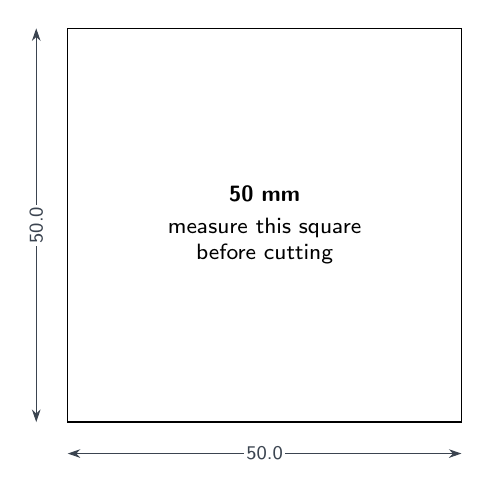
\begin{tikzpicture}[x=1mm,y=1mm]
    \draw[line width=0.5pt] (0,0) rectangle (50,50);
    \node[align=center,font=\footnotesize] at (25,25) {\textbf{50 mm}\\[2pt]measure this square\\before cutting};
    \draw[dim] (0,-4) -- (50,-4) node[dimlabel]{50.0};
    \draw[dim] (-4,0) -- (-4,50) node[dimlabel]{50.0};
  \end{tikzpicture}}

\newcommand{\code}[1]{\texttt{#1}}
\newcommand{\fig}[1]{Figure~\ref{#1}}

% ── running header and footer
\pagestyle{fancy}
\fancyhf{}
\renewcommand{\headrulewidth}{0.4pt}
\renewcommand{\headrule}{\hbox to\headwidth{\color{rule}\leaders\hrule height \headrulewidth\hfill}}
\fancyhead[L]{\footnotesize\color{muted}\doctitle}
\fancyhead[R]{\footnotesize\color{muted}radar-dev · 2.4 GHz FMCW radar}
\fancyfoot[L]{\footnotesize\color{muted}Sizes in mm unless marked. Generated from antenna/tools/horn.py and the 3-D model.}
\fancyfoot[R]{\footnotesize\color{muted}\thepage}
\fancypagestyle{plain}{\fancyhf{}\fancyfoot[R]{\footnotesize\color{muted}\thepage}\renewcommand{\headrulewidth}{0pt}}

% generated by tools/make_figures.py — do not edit
\newcommand{\aperW}{263.8}
\newcommand{\aperH}{193.1}
\newcommand{\pipeW}{86.4}
\newcommand{\pipeH}{43.2}
\newcommand{\flareL}{91.5}
\newcommand{\pipeL}{115}
\newcommand{\probeZ}{43.7}
\newcommand{\probeLen}{28}
\newcommand{\rodCut}{32}
\newcommand{\seam}{147.9}
\newcommand{\hTop}{118.3}
\newcommand{\hSide}{127.5}
\newcommand{\wideW}{87.5}
\newcommand{\backW}{88.5}
\newcommand{\backH}{44.3}
\newcommand{\tabW}{6}
\newcommand{\gain}{13.4}
\newcommand{\hpE}{34.2}
\newcommand{\hpH}{36.2}
\newcommand{\boardW}{457}
\newcommand{\boardD}{381}
\newcommand{\upH}{530.8}
\newcommand{\upX}{213}
\newcommand{\upCC}{426}
\newcommand{\beamLen}{444}
\newcommand{\beamRXlen}{408}
\newcommand{\beamRXtop}{252.8}
\newcommand{\beamTXtop}{542.8}
\newcommand{\rxY}{300}
\newcommand{\txY}{590}
\newcommand{\hornBase}{193.1}
\newcommand{\rowGap}{26.2}
\newcommand{\braceLen}{242.2}
\newcommand{\saddleW}{56.2}
\newcommand{\saddleGap}{48.2}
\newcommand{\saddleD}{34}
\newcommand{\saddleH}{32}
\newcommand{\saddleBehind}{90}
\newcommand{\overhang}{36}
\newcommand{\screenW}{293.1}
\newcommand{\screenH}{130}
\newcommand{\braceFootX}{128}
\newcommand{\txTop}{721.9}
\newcommand{\frontToFrame}{145.5}
\newcommand{\beamRXbottom}{240.8}
\newcommand{\braceTop}{226.8}
\newcommand{\leanTop}{39}
\newcommand{\leanSide}{44}
\newcommand{\cornerBend}{64}
\newcommand{\braceAngle}{69}
\newcommand{\sheetPct}{62}
\newcommand{\sheetIn}{178}

% table rows from a file: the primitive \input, because LaTeX's is not expandable inside a tabular
\makeatletter\newcommand{\rowsfrom}[1]{\@@input generated/#1.tex }\makeatother
\newcolumntype{Y}{>{\centering\arraybackslash}X}
